\documentclass[a4paper,man,natbib]{apa6}

\usepackage[english]{babel}
\usepackage[utf8x]{inputenc}
\usepackage{amsmath}
\usepackage{graphicx}
\usepackage[colorinlistoftodos]{todonotes}

\title{Title}
\shorttitle{short title}
\author{Benjamin Floyd}
\affiliation{University of Virginia}

%\abstract{Your abstract here.}

\begin{document}
\maketitle

\section{Introduction}
\label{sec:intro}

In the field of Computer Science (CS), gender disparity has been a challenge for
over 40 years [FIXME:CITE]. Specifically, women are typically underrepresented
in the field. Today, the number of women in undergraduate Computer Science
programs hovers around 18\%, nationally [FIXME:CITE]. Computer Science
departments traditionally have trouble recruiting female students; this
accounts for some of the gender disparity. However, departments also suffer
from attrition of female students once they enter the major. A reason commonly
cited among females who decide to leave the major is that they
under-perform in introductory classes. Loosely, this claim admits two broad
possibilities: either female students actually under-perform in introductory
courses, or they only perceive that they under-perform. This paper considers
each of these possibilities in turn. First, we investigate if female students
actually perform worse than their male peers in introductory classes. We
conclude that there is no evidence to support the claim that females
under-perform in this regard. Second, we investigate if females perceive that
they are under-performing and consider possible causes of this perception.
To explore these questions, we analyze survey and grade data for over one
thousand students across CS1 and CS2 courses.

\section{Methods}
\label{sec:methods}
To address the research questions, we analyze two sources of data: anonymous
surveys, and student grade information. 

\subsection{Surveys}
\label{sec:survey}
Students answered an IRB approved, web-based survey with approximately ten
questions. The survey included demographic questions, Likert-scale questions,
and free-form questions. The surveys were applied at various points such as the
beginning of a course, the end of a course, or when dropping a class. Students
were tracked through an anonymous identifier in order to recognize when the
same student takes the survey more than once. The dataset contains responses
from 1019 distinct undergraduate students who were enrolled in Computer Science
introductory courses between 2008 and 2010 at the University of Virginia.

\subsection{Grades}
\label{sec:grade}
Instructors provided final grade and gender data for 1,023 distinct
undergraduates who were enrolled in CS1 or CS2 courses between 2008 and 2010 at
the University of Virginia. This amounted to a total of 2,021 final grade
instances. Student genders were manually labelled as male, female, or unknown
based on name and photograph information. Letter grades were converted to the
standard College Board GPA scale (i.e. "B"=3.0, "B+"=3.3, etc.). Final grades
marked as either "incomplete" or "pass/fail" were omitted from the dataset (41
out of 2062 were not included). Figure [FIXME] shows the classes involved in
the creation of this dataset, as well as the sample sizes for each year. The
University of Virginia CS Department features two different CS1 classes based
on intended degree; additionally, the CS2 class is considered introductory. 

Because of the anonymous nature of the surveys, it was impossible to link a
particular survey respondent to a set of CS course grades.

\section{Results}
\label{sec:results}
We address two primary research questions by analyzing the dataset described in
the Methods section. These questions correspond to two broad explanations for
why female students report under-performing in introductory CS courses. First,
we evaluate whether female student actually perform worse that their male peers
in these courses; we find no evidence to support the claim that females perform
worse than males in this regard. Then, we investigate if females only perceive
that they are under-performing, and discuss possible factors that contribute to
this perception. 

\subsection{RQ1: Do females under-perform their male peers in introductory CS classes?}




\subsection{References}

LaTeX automatically generates a bibliography in the APA style from your .bib file. The citep command generates a formatted citation in parentheses \citep{Lamport1986}. The cite command generates one without parentheses. LaTeX was first discovered by \cite{Lamport1986}.

\subsection{Tables and Figures}

Use the table and tabular commands for basic tables --- see Table~\ref{tab:widgets}, for example. You can upload a figure (JPEG, PNG or PDF) using the files menu. To include it in your document, use the includegraphics command as in the code for Figure~\ref{fig:frog} below.

% Commands to include a figure:
\begin{figure}
\centering
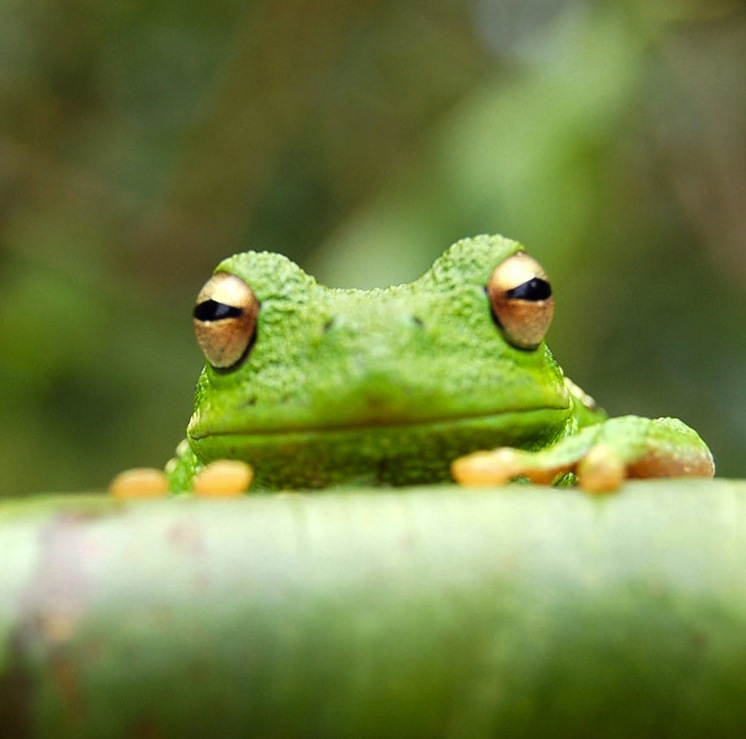
\includegraphics[width=0.5\textwidth]{frog.jpg}
\caption{\label{fig:frog}This is a figure caption.}
\end{figure}

\begin{table}
\centering
\begin{tabular}{l|r}
Item & Quantity \\\hline
Widgets & 42 \\
Gadgets & 13
\end{tabular}
\caption{\label{tab:widgets}An example table.}
\end{table}

\subsection{Mathematics}

\LaTeX{} is great at typesetting mathematics. Let $X_1, X_2, \ldots, X_n$ be a sequence of independent and identically distributed random variables with $\text{E}[X_i] = \mu$ and $\text{Var}[X_i] = \sigma^2 < \infty$, and let
$$S_n = \frac{X_1 + X_2 + \cdots + X_n}{n}
      = \frac{1}{n}\sum_{i}^{n} X_i$$
denote their mean. Then as $n$ approaches infinity, the random variables $\sqrt{n}(S_n - \mu)$ converge in distribution to a normal $\mathcal{N}(0, \sigma^2)$.

\subsection{Lists}

You can make lists with automatic numbering \dots

\begin{enumerate}
\item Like this,
\item and like this.
\end{enumerate}
\dots or bullet points \dots
\begin{itemize}
\item Like this,
\item and like this.
\end{itemize}

We hope you find write\LaTeX\ useful, and please let us know if you have any feedback using the help menu above.

\bibliography{example}

\end{document}

%
% Please see the package documentation for more information
% on the APA6 document class:
%
% http://www.ctan.org/pkg/apa6
%
